\documentclass{article}

\usepackage{graphicx}
\usepackage{tikz}
\usepackage{tikzsymbols}
\usetikzlibrary{calc,patterns,shapes.geometric}
\pagestyle{empty}
\usepackage[margin=0pt]{geometry}
\geometry{papersize={14in,12in}}

\def\centerarc[#1](#2)(#3:#4:#5){\draw[#1] ($(#2)+({#5*cos(#3)},{#5*sin(#3)})$) arc (#3:#4:#5);}

\begin{document}
	\begin{figure}
		\centering
		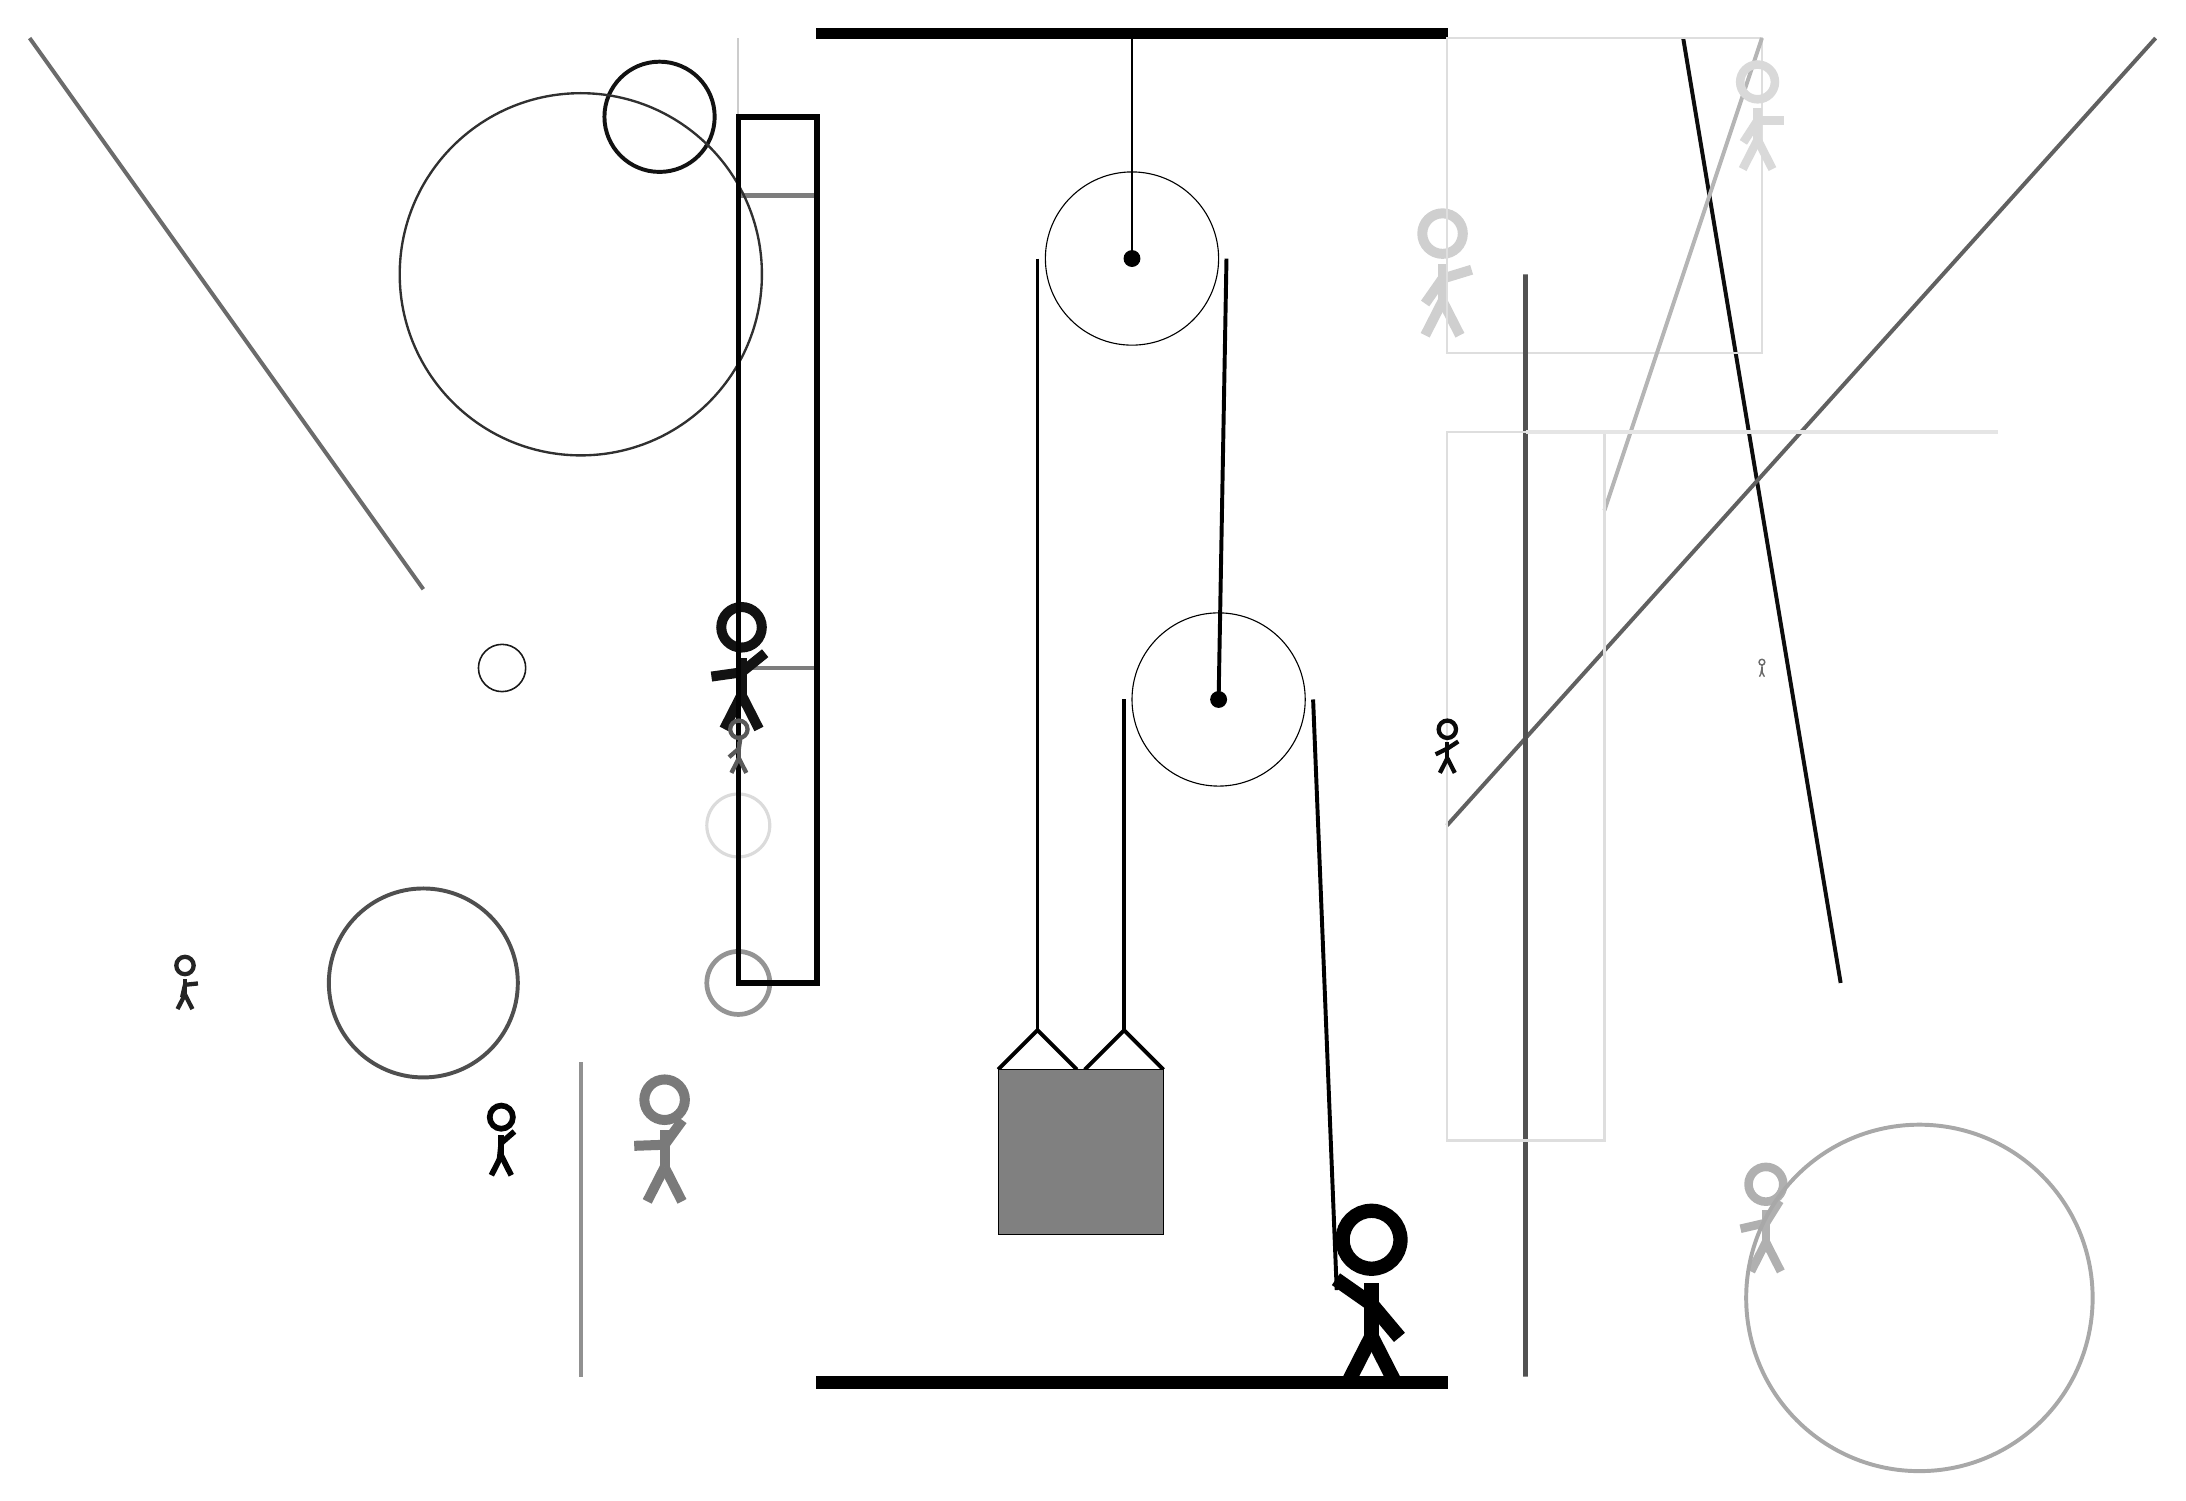
\begin{tikzpicture}
			%%%%% START %%%%%
			
			\draw[fill=black] (-2, 14) rectangle (6, 14.125);
			
			\draw (2, 11.2) circle (1.1);
			\draw[fill=black] (2, 11.2) circle (0.1);
			\draw[thick] (2, 11.2) -- (2, 14);
			
			\draw (3.1, 5.6) circle (1.1);
			\draw[fill=black] (3.1, 5.6) circle (0.1);
			
			\draw[line width = 0.5mm]  (0.3, 0.9) -- (0.8, 1.4) -- (1.3, 0.9);
			\draw[line width = 0.5mm]  (1.4, 0.9) -- (1.9, 1.4) -- (2.4, 0.9);
			\draw[fill=black!50] (0.3, 0.9) rectangle (2.4, -1.2);
			
			\draw [line width=0.2mm, color=black!90](-6, 6) circle (0.3);
			
			\draw[line width=0.5mm, color=black!95](11, 2) -- (9, 14);
			\draw[line width=0.6mm, color=black!51] (-3, 6) rectangle (-2, 12);
			\node[line width=0.7mm, color=black!31] at (10, -1) {\Strichmaxerl[6][13][58]};
			
			\draw [line width=0.5mm, color=black!93](-4, 13) circle (0.7);
			
			\node[line width=0.2mm, color=black!19] at (6, 11) {\Strichmaxerl[7][55][17]};
			\draw [line width=0.6mm, color=black!42](-3, 2) circle (0.4);
			\draw[line width=0.3mm, color=black!13] (6, 14) rectangle (10, 10);
			\draw [line width=0.5mm, color=black!34](12, -2) circle (2.2);
			\draw [line width=0.5mm, color=black!69](-7, 2) circle (1.2);
			\draw[line width=0.5mm, color=black!29](8, 8) -- (10, 14);
			
			\draw[line width=0.5mm, color=black!43](-5, -3) -- (-5, 1);
			\node[line width=0.6mm, color=black!15] at (10, 13) {\Strichmaxerl[6][57][0]};
			\node[line width=0.6mm, color=black!99] at (-6, 0) {\Strichmaxerl[4][84][41]};
			\draw[line width=0.5mm, color=black!62](6, 4) -- (15, 14);
			\node[line width=0.3mm, color=black!58] at (10, 6) {\Strichmaxerl[1][77][88]};
			
			\draw[line width=0.7mm, color=black!68] (7, -3) rectangle (7, 11);
			
			\draw[line width=0.3mm, color=black!13] (8, 0) rectangle (6, 9);
			\draw [line width=0.3mm, color=black!81](-5, 11) circle (2.3);
			\draw[line width=0.3mm, color=black!20] (-3, 14) rectangle (-3, 13);
			\draw[line width=0.5mm, color=black!58](-7, 7) -- (-12, 14);
			
			\draw [line width=0.4mm, color=black!14](-3, 4) circle (0.4);
			\node[line width=0.4mm, color=black!52] at (-4, 0) {\Strichmaxerl[7][2][54]};
			\draw[line width=0.6mm, color=black!78] (-3, 12) rectangle (-3, 13);
			\draw[line width=0.5mm, color=black!10](7, 9) -- (13, 9);
			\node[line width=0.6mm, color=black!86] at (-10, 2) {\Strichmaxerl[3][77][6]};
			\node[line width=0.3mm, color=black!93] at (-3, 6) {\Strichmaxerl[7][8][39]};
			\draw[line width=0.7mm, color=black!99] (-2, 13) rectangle (-3, 2);
			\node[line width=0.3mm, color=black!65] at (-3, 5) {\Strichmaxerl[3][41][82]};
			\node[line width=0.3mm, color=black!96] at (6, 5) {\Strichmaxerl[3][26][33]};
			
			\draw[line width = 0.5mm] (0.8, 11.2) -- (0.8, 1.4);
			\centerarc[line width = 0.5mm](2, 11.2)(0:180:1.2000000000000002);
			\draw[line width = 0.5mm] (3.2, 11.2) -- (3.1, 5.6);
			\draw[line width = 0.5mm] (1.9, 5.6) -- (1.9, 1.4);
			\centerarc[line width = 0.5mm](3.1, 5.6)(0:180:1.2000000000000002);
			\draw[line width = 0.5mm] (4.3, 5.6) -- (4.6, -1.9);
			
			\node at (5, -2) {\Strichmaxerl[10][-35][-50]};
			
			\draw[fill=black] (-2, -3) rectangle (6, -3.15);
			
			%%%%% END %%%%%
		\end{tikzpicture}
	\end{figure}	
\end{document}